% !TeX spellcheck = en_US
\documentclass[a4paper,11pt]{scrartcl}

%\renewcommand{\arraystretch}{1.5}


%\lvsemester{SS 2021}
%\lvname{Computational Linguistics}
%\zeit{60 minutes}
%\datum{July 21\textsuperscript{th} 2021}

\usepackage{graphicx}
\graphicspath{
    {.} % document root dir
    {images/}
}


\usepackage{enumitem}
\usepackage[outputdir=out]{minted}
\usepackage{xcolor} % to access the named colour LightGray
\definecolor{LightGray}{gray}{0.9}


% Load the setspace package
\usepackage{setspace}
% Using \doublespacing in the preamble 
% changes text to double line spacing
\doublespacing


\title{W6 Assignment -- Machine Learning 1}
\subtitle{Computational Linguistics}

\author{John Gamboa}
\date{\today}

\setkomafont{author}{\sffamily}
\setkomafont{date}{\sffamily}



\setlength{\parindent}{0pt}



\begin{document}
\maketitle

\section{k Nearest Neighbor Classifier}

\subsection{Behavior}

Consider the image below:

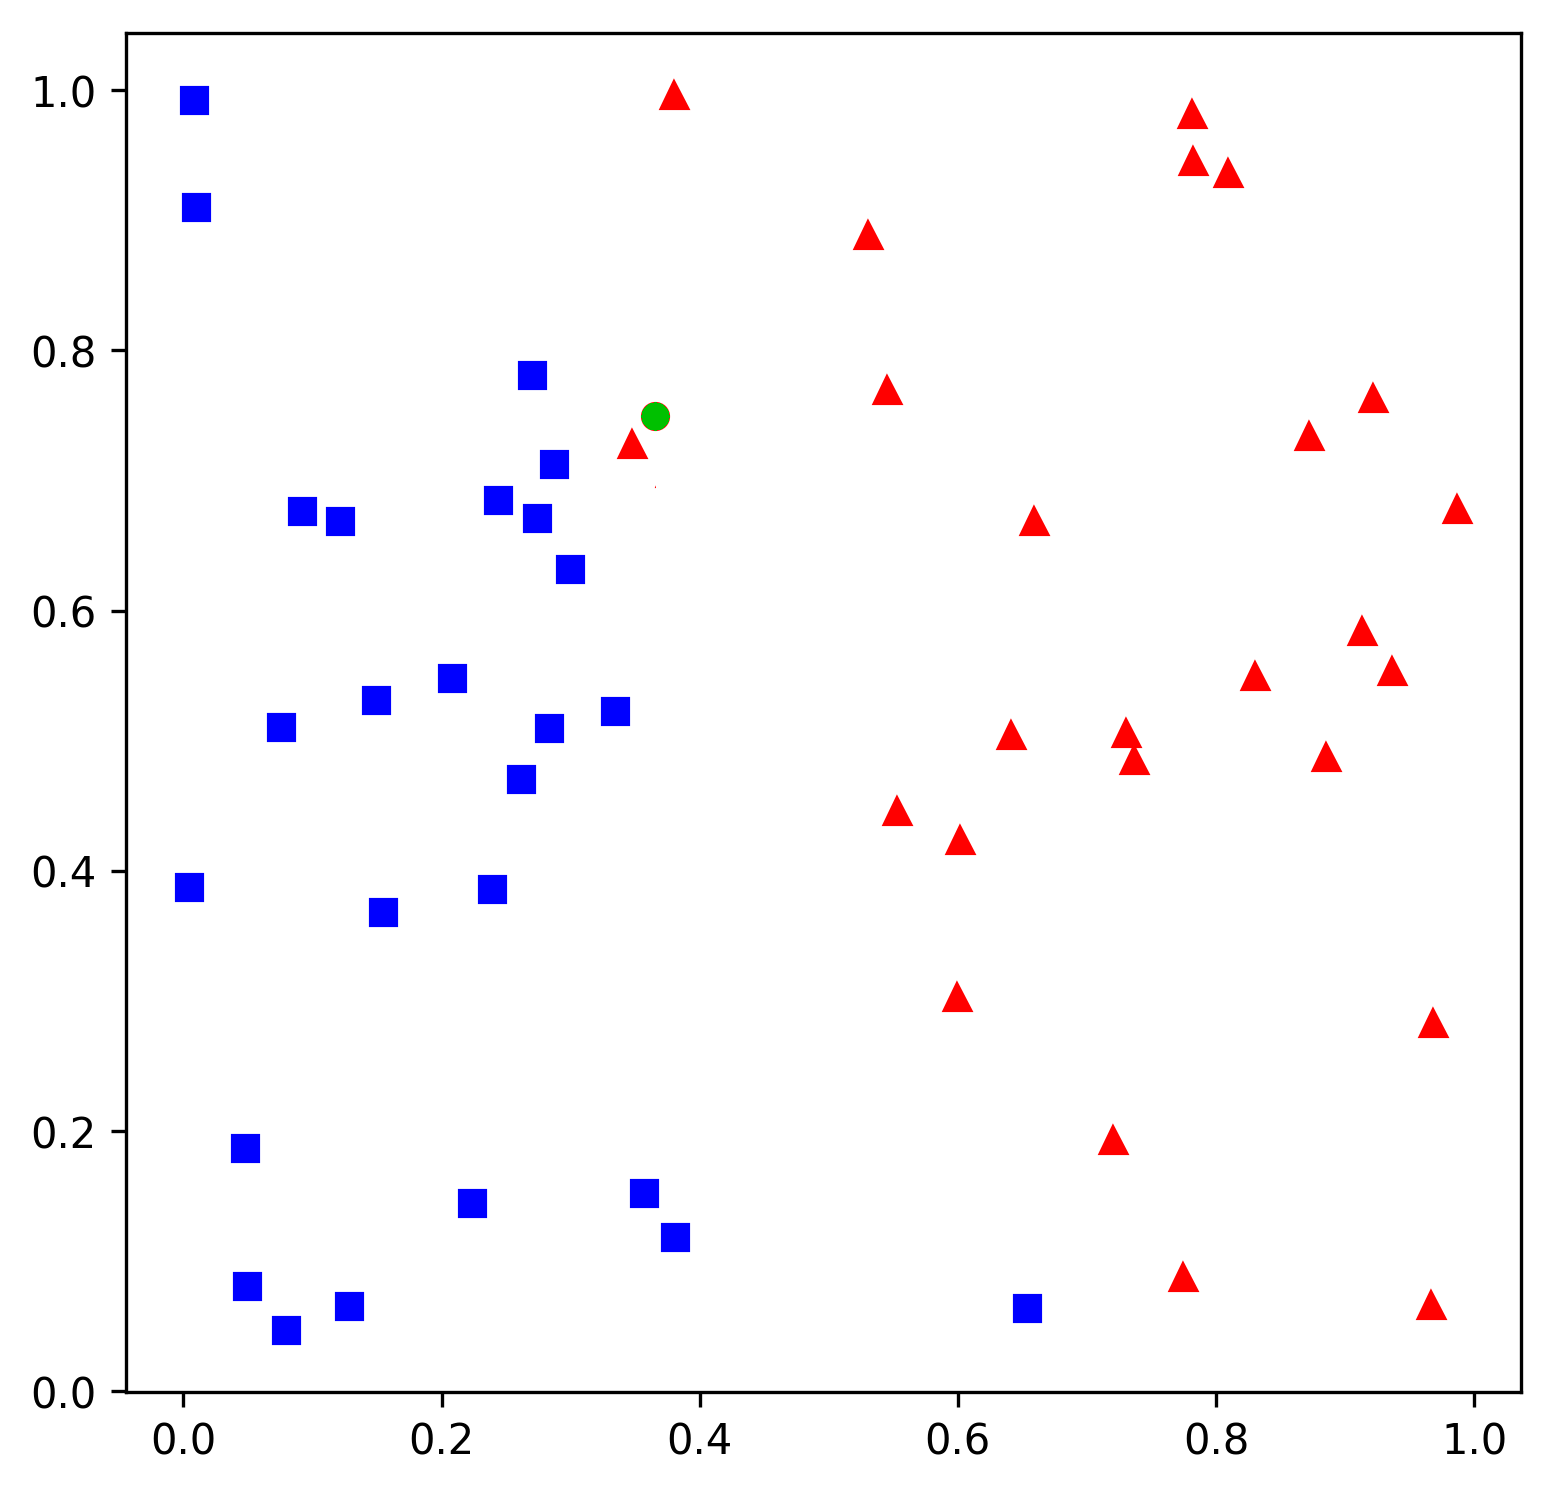
\includegraphics[width=0.6\textwidth]{reds_and_blues}

Assume that the training data consists of all red and blue dots and the test
data consists uniquely of the green dot. Our goal is to classify the green dot.
In this context, one could say that... (answer \textit{TRUE} or \textit{FALSE})

\begin{itemize}
\singlespacing
\item When k=1, the kNN classifier would output ``red";

\verb|answer|: \_\_\_\_\_\_\_\_\_\_\_\_\_\_\_\_\_\_\_\_\_\_\_\_\_\_\_\_\_\_\_\_

\item When k=3, the kNN algorithm would invariably output ``blue";

\verb|answer|: \_\_\_\_\_\_\_\_\_\_\_\_\_\_\_\_\_\_\_\_\_\_\_\_\_\_\_\_\_\_\_\_

\item When k=3, the kNN classifier that doesn't take distances into account
      would output ``blue";

\verb|answer|: \_\_\_\_\_\_\_\_\_\_\_\_\_\_\_\_\_\_\_\_\_\_\_\_\_\_\_\_\_\_\_\_

\item When k=6, the kNN algorithm would output ``red";

\verb|answer|: \_\_\_\_\_\_\_\_\_\_\_\_\_\_\_\_\_\_\_\_\_\_\_\_\_\_\_\_\_\_\_\_

\item When k=2, the kNN algorithm would invariably output ``red".

\verb|answer|: \_\_\_\_\_\_\_\_\_\_\_\_\_\_\_\_\_\_\_\_\_\_\_\_\_\_\_\_\_\_\_\_
\end{itemize}


\subsection{Distance Measures}

Calculate the Euclidean Distance between the following points:

\begin{itemize}
\singlespacing
\item $a = (1,1,1),  b = (1,1,10)$
      \verb|answer|: \_\_\_\_\_\_\_\_\_\_\_\_\_\_\_\_\_\_\_\_\_\_\_\_\_\_\_\_\_\_\_

\item $a = (1,1,1),  b = (1,10,1)$
      \verb|answer|: \_\_\_\_\_\_\_\_\_\_\_\_\_\_\_\_\_\_\_\_\_\_\_\_\_\_\_\_\_\_\_

\item $a = (1,1,1),  b = (10,1,1)$
      \verb|answer|: \_\_\_\_\_\_\_\_\_\_\_\_\_\_\_\_\_\_\_\_\_\_\_\_\_\_\_\_\_\_\_

\item $a = (1,1,1),  b = (1,2,2)$
      \verb|answer|: \_\_\_\_\_\_\_\_\_\_\_\_\_\_\_\_\_\_\_\_\_\_\_\_\_\_\_\_\_\_\_

\item $a = (1,1,1),  b = (2,2,2)$
      \verb|answer|: \_\_\_\_\_\_\_\_\_\_\_\_\_\_\_\_\_\_\_\_\_\_\_\_\_\_\_\_\_\_\_
\end{itemize}

Notice how it varies when only one dimension has changed, when two
dimensions have changed, and three dimensions have changed. It may be helpful
to plot these into a 3D space and see why this is the case.
 

Calculate the Manhattan Distance between the following points:

\begin{itemize}
\singlespacing
\item $a = (1,1,1),  b = (1,1,10)$
      \verb|answer|: \_\_\_\_\_\_\_\_\_\_\_\_\_\_\_\_\_\_\_\_\_\_\_\_\_\_\_\_\_\_\_

\item $a = (1,1,1),  b = (1,10,1)$
      \verb|answer|: \_\_\_\_\_\_\_\_\_\_\_\_\_\_\_\_\_\_\_\_\_\_\_\_\_\_\_\_\_\_\_

\item $a = (1,1,1),  b = (10,1,1)$
      \verb|answer|: \_\_\_\_\_\_\_\_\_\_\_\_\_\_\_\_\_\_\_\_\_\_\_\_\_\_\_\_\_\_\_

\item $a = (1,1,1),  b = (1,2,2)$
      \verb|answer|: \_\_\_\_\_\_\_\_\_\_\_\_\_\_\_\_\_\_\_\_\_\_\_\_\_\_\_\_\_\_\_

\item $a = (1,1,1),  b = (2,2,2)$
      \verb|answer|: \_\_\_\_\_\_\_\_\_\_\_\_\_\_\_\_\_\_\_\_\_\_\_\_\_\_\_\_\_\_\_
\end{itemize}

Notice how the variability of the Euclidean Distance is not present
anymore. Can you see why this is the case?


\section{Evaluation}

Let's say we created a classifier that receives a new data point and produces
a color indicating the class of that point. Now we want to check how well it
performs for new data, that was just collected. Let's say our newly collected
data had the following labels:

\begin{minted}[bgcolor=LightGray,fontsize=\footnotesize]{python}
[red, red, red, blue, red, green, green, gray, red, blue, grey, red]
\end{minted}

But the classifier actually produced the following labels:

\begin{minted}[bgcolor=LightGray,fontsize=\footnotesize]{python}
[red, green, red, blue, red, blue, green, gray, red, grey, grey, red]
\end{minted}

Calculate accuracy:

\verb|answer|: \_\_\_\_\_\_\_\_\_\_\_\_\_\_\_\_\_\_\_\_\_\_\_\_\_\_\_\_\_\_\_\_


\section{Bag of Words}

Let's say we were given the following sentence:

\begin{minted}[bgcolor=LightGray,fontsize=\footnotesize]{text}
The quick brown fox jumped over the lazy dog.
The dog was lazy and therefore didn't care about it
\end{minted}

We want to create a 3-words vocabulary (plus ``UNK'') for this sentence,
and represent it with a bag of words.
Write the Bag of Words representation:
(use a list of numbers, and no spaces. E.g., [3,5,2,8])

\verb|answer|: \_\_\_\_\_\_\_\_\_\_\_\_\_\_\_\_\_\_\_\_\_\_\_\_\_\_\_\_\_\_\_\_


\end{document}

